
\subsection{Minimale Netzkonfiguration}
Bei fast allen Betriebssystemen m"ussen w"ahrend der Installation ein paar
Angaben gemacht werden, die "uberall gleichartig sind. In den meisten
Fällen sollte es dabei reichen, wenn man in den Netzwerkeinstellungen
,,IP-Adresse automatisch beziehen'', ,,DHCP verwenden'' oder ähnliches
auswählt. Die Einzelheiten werden für die verschiedenen
Betriebssysteme im Folgenden beschrieben.
\subsubsection{Windows XP}
Man klickt sich durch  über \fbox{Startmenü} $\Rightarrow$
\fbox{Einstellungen} $\Rightarrow$ \fbox{Systemsteuerung} zum Fenster
\fbox{Netzwerkverbindungen} durch:
\centergraphics{netzwerkverbindungen}
%insert screenshot
Hier ist nun die richtige Netzwerkverbindung auszuwählen. Wie man sie
ermittelt, wird im Abschnitt zur MAC-Adresse beschrieben. Zunächst
sollte man ihren Status überprüfen:  Die Netzwerkverbindung muss
aktiviert sein. Andernfalls muss sie mittels
\fbox{Rechtsklick}$\Rightarrow$\fbox{Aktivieren} aktiviert
werden.  Anschließend ruft man mit
\fbox{Rechtsklick}$\Rightarrow$\fbox{Eigenschaften} das linke Fenster auf:  
\begin{center}
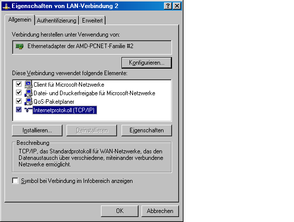
\includegraphics{eigenschaften_xp}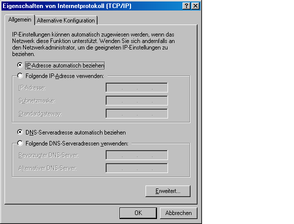
\includegraphics{dhcp_xp}    
\end{center}
 

Hier ist nun auf \fbox{Internetprotokoll (TCP/IP)} und anschließend
auf \fbox{Eigenschaften} zu klicken. Es sollte sich das rechte Fenster
öffnen.
%und noch einer
Die Einstellungen sollten mit den abgebildeten
übereinstimmen. Andersweitig sind sie zu ändern und mit einen
beherzten Klick auf \fbox{Ok} zu bestätigen. Damit sollte dann in der
Tat alles ok sein.
\subsubsection{Windows Vista}

\subsubsection{Windows 7}

\subsubsection{Linux}
\small{Wie schon bei der MAC-Adresse gilt: Je nach Distribution kann es kleinere Unterschiede
geben. Die folgende Anleitung wurde für Debian und Ubuntu getestet und
sollte sich leicht an andere Distributionen anpassen lassen.}
Die folgenden Einstellungen müssen als Administrator (,,root'') vorgenommen
werden. Je nach Distribution ist es dazu erforderlich, sich als root
anzumelden, oder anderweitig als Administrator auszuweisen. In Ubuntu
erfolgt dies beispielsweise mit Hilfe des Programms sudo.\\\\
Die Einstellungen werden durch Bearbeiten der Datei
\texttt{/etc/network/interfaces} vorgenommen. Sie sollte danach
folgende Einträge erhalten:
\begin{verbatim}
# The loopback network interface
auto lo 
iface lo inet loopback
# The primary network interface
auto eth1
iface eth1 inet dhcp 
\end{verbatim}
Dabei muss \texttt{eth1} durch das Kürzel der jeweiligen Netzwerkkarte
ersetzt werden. Wie man diese Netzwerkkarte herausfindet ist im
Abschnitt zur MAC-Adresse beschrieben. Anschließend muss man diese
Änderungen noch aktivieren. Dazu gibt man in eine Konsole nacheinander
folgende Befehle ein:
\begin{verbatim}
ifdown eth1
ifup eth1
\end{verbatim}
Wieder muss \texttt{eth1} durch das entsprechende Kürzel ersetzt
werden. Damit ist die Konfiguration erledigt.

\subsubsection{Testen des Anschlusses}
Sind die Einstellungen erledigt, sollte man die Einstellung
testen. In den meisten Fällen sollte alles klappen. Sollte dies nicht
der Fall sein, gibt es folgende Möglichkeiten: Die mit Abstand
häufigste Fehlerquelle ist es, bei der Anmeldung eine falsche
MAC-Adresse angegeben zu haben. Es empfiehlt sich nun, die
Anmeldebestätigung herauszusuchen und die dort angegebene MAC-Adresse
mit der tatsächlichen zu vergleichen. Sollte man sie vergessen haben
(nicht sooo überraschend bei einer Folge aus hexadezimalen Ziffern),
kann man sie ja mit den aus Abschnitt \ref{sec:netzw-und-mac}
genannten Methoden erneut ermitteln. Sollte sie falsch sein, kann man
die Richtige den Admins in der Sprechstunde oder über eine Email an
\url{admin@schunternet.de} mitteilen\footnote{Wie soll das gehen ohne
  Internet? Hier ist nun Fantasie gefragt: Vom Fragen des Nachbarn,
  über die Computerräume der Uni gibt es ein breites Feld an
  Möglichkeiten :)}.\\\\
Ein anderer häufiger Fehler ist das Benutzen des zweiten
Anschlusses. Jedes Zimmer ist mit einer Dose mit zwei Anschlüssen
ausgestattet. Die Zweite ist im Normalfall aber nicht
freigeschaltet. Dieses Problem sollte sich aber schnell beheben
lassen. Stellenweise sind einige Dosen auch falsch angeschlossen
worden. In so einen Fall sollte man umgehend einen der Hausmeister und
uns informieren, damit entsprechend Abhilfe geschaffen werden
kann.\\\\
Können alle diese Fehler ausgeschlossen werden, kann man sein Glück
mit der manuellen Konfiguration der Netzwerkkarte versuchen. Und
natürlich ist die Sprechstunde kein Selbstzweck, sondern durchaus
dafür da, Probleme anzusprechen und dann auch zu lösen :)

\subsection{Manuelle Konfiguration der Netzwerkkarte}
Eine Anmerkung vorweg: Im Normallfall sollten die folgenden Schritte
gar nicht nötig sein, da im Netzwerk ein DHCP-Server arbeitet, der
alles automatisch erledigt. Allerdings kann es sehr selten dazu
kommen, dass dieser seinen Geist aufgibt. Auch zur Fehlersuche können
sie hilfreich sein. Aber: \textbf{\Large Sie sollten nur getätigt werden, wenn man
genau weiss was man tut!!! Ein Fehler kann zur Sperre führen!!!} Der
Hintergrund ist, dass zur Vermeidung von Mißbrauch einer unser Server
eine Art Abwehrprogramm laufen lässt. Dieses Programm bemerkt
 enventuelle Angriffe und sperrt dann den entsprechenden
Rechner. Aus technischer Sicht ist ein Mißbrauch und ein Fehler aber
nicht zu unterscheiden. Daher nochmal der Hinweis: \textbf{\Large Folgendes nur
  tun, wenn man sich seiner Sache ganz sicher ist!!! Ansonsten wird
  gerne in der Sprechstunde weitergeholfen!}.\\\\

\subsubsection{Benötigte Daten}
Die nötigen Daten sind auf der Anmeldebestätigung vermerkt, die man
nach der Freischaltung des Anschlusses erhalten hat. Sie werden im
folgenden näher erläutert:
\begin{description}
  \item[TCP/IP--Adresse bzw. Host--Adresse] hier muss die sogenannte IP--Adresse
    des eigenen Rechners eingegeben werden, z.B. 134.169.168.255. 

    Jeder Computer im Wohnheim hat eine eigene IP--Adresse. Dies sind vier
    Zahlen von 0 bis 255 die jeweils durch einen Punkt getrennt werden. Die
    ersten beiden Zahlen sind innerhalb des Wohnheims (und innerhalb der TU)
    immer gleich und zwar 134.169. Die dritte Zahl ist im Wohnheim entweder
    168 oder 169. 
%    Zun"achst werden die Adressen aus dem Bereich 134.169.168
%    vergeben, der Bereich 134.169.169 ist f"ur wachsende Teilnehmerzahlen
%    reserviert. 
    Die IP--Adresse identifiziert genau einen Computer, also hat jeder Rechner
    eine andere IP--Adresse. Diese wird euch bei Annahme des Antrags von
    der \glossar Administration mitgeteilt.

    Hier wurde von dem Beispiel 134.169.168.255 ausgegangen. Anstatt der 255
    muss dann die passende/richtige Endung eingesetzt werden. 

  \item[Subnet mask] Hier muss korrekterweise 255.255.254.0 eingegeben
    werden.

  \item[Netzadresse, Broadcast] Wenn danach gefragt wird, muss als Netzadresse
    134.169.168.0 und als Broadcastadresse 134.169.169.255 eingetragen werden.

  \item[DNS/Name Server, Router, Gateway] Hier muss immer die
    IP--Adresse 134.169.168.1 eingegeben werden.
 
  \item[TCP/IP Domain Name] Hier muss \url{schunter.etc.tu-bs.de} eingegeben
    werden.

  \item[Host Name oder Rechnername] Hier muss der im Antrag angegebene
    Rechnername (siehe auch \ref{ip}) eingetragen werden.
 
%  \item[DHCP, BOOTP und DDNS] Falls hiernach gefragt wird, dann sollte dies
%    nicht ausgew"ahlt bzw.\  mit nein beantwortet werden.
\end{description}

Ansonsten folgen hier noch ein paar Hinweise, die betriebssystemspezifisch
sind.
\subsubsection{Windows XP}
Zunächst öffne man wieder mittels \fbox{Startmenü} $\Rightarrow$
\fbox{Einstellungen} $\Rightarrow$ \fbox{Systemsteuerung} das Fenster
\fbox{Netzwerkverbindungen}. Nach Überprüfung des Status der richtigen
Netzwerkverbindung, öffne man mit \fbox{Rechtsklick} $\Rightarrow$
\fbox{Einstellungen} folgendes Fenster:

Hier ist nun auf \fbox{Internetprotokoll (TCP/IP)} und anschließend
auf \fbox{Eigenschaften} zu klicken. Es sollte sich nun ein neues
Fenster öffnen, in dem man die Daten von der Anmeldebestätigung
eintragen kann:
\centergraphics{manu_xp}
Dabei sind statt der abgebildeten Daten natürlich die aauf der
Bestätigung abgedruckten
einzutragen. 
% \subsubsection{Windows95/98}

% Damit also auf zur Maus--Klick--Orgie: Es wird davon ausgegangen, da"s das
% Fenster "`Systemsteuerung"' ge"offnet ist (zu finden "uber das Men"u \fbox{Start}
% unter \fbox{Einstellungen}).

% Zun"achst zur Netzwerkkarte und damit zum
% schwierigsten Teil: Wann die Karte konfliktfrei l"auft und Windows95 auch
% "uberzeugt davon ist, ist nur sehr schwer festzustellen. Das hier sind einige
% Anhaltspunkte.

% \centergraphics[width=13.5cm]{W95Netzkarte.eps}

% Die Karte funktioniert mit Sicherheit noch nicht, wenn
% \begin{itemize}
%   \item sie unter \fbox{System} $\Rightarrow$ \fbox{Ger"atemanager}
%     $\Rightarrow$ \fbox{Netzwerkkarten} gar nicht auftaucht oder
%   \item das Netzwerkkartensymbol an besagter Stelle mit einem gelb unterlegten
%     Rufzeichen \raisebox{0.4mm}{$\bigcirc$}\hspace{-2.7mm}!\ \ versehen ist.
% \end{itemize}

% Die Karte funktioniert mit sehr gro"ser Wahrscheinlichkeit, wenn 
% \begin{itemize}
%   \item sie unter \fbox{System} $\Rightarrow$ \fbox{Ger"atemanager}
%     $\Rightarrow$ \fbox{Netzwerkkarten} auftaucht und
%   \item nicht mit dem gelben Symbol versehen ist und 
%   \item sie unter \fbox{System} $\Rightarrow$ \fbox{Ger"atemanager}
%     $\Rightarrow$ \fbox{Computer} $\Rightarrow$ \fbox{Eigenschaften} nicht mit
%     dem kleinen runden \raisebox{0.2mm}{$\bigcirc$}\hspace{-2.7mm}i~--Symbol
%     (blau auf wei"sem Grund) versehen ist.
% \end{itemize}

% \centergraphics{W95TCPIP.eps}

% Falls alle Bedingungen bis auf die letzte erf"ullt sind, kann die Karte
% m"oglicherweise auch funktionieren. In dem Fall hilft nur Ausprobieren. Aus
% meinen Erfahrungen kann ich leider keine zielgerichtete Anleitung
% zusammenstricken, wie auftretende Konflikte beseitigt werden, aber
% funktioniert hat es letztendlich doch immer irgendwie.
% Oft ist auch Gl"uck bzw. Willk"ur seitens des Betriebssystemherstellers dabei.
% Wenn die Karte einmal installiert ist, ist der Rest ein
% Kinderspiel. 

% Unter \fbox{Netzwerk} wird durch \fbox{Hinzuf"ugen} $\Rightarrow$
% \fbox{Protokoll} $\Rightarrow$ \fbox{Hinzuf"ugen} $\Rightarrow$
% \fbox{Microsoft} $\Rightarrow$ \fbox{TCP/IP} $\Rightarrow$ \fbox{OK} das
% TCP/IP--Protokoll installiert. "Uber \fbox{TCP/IP} $\Rightarrow$
% \fbox{Eigenschaften} werden die oben genannten Einstellungen (IP--Adresse,
% \glossar Subnetmask, Gateway, \glossar DNS--Server, Host-- und Domain--Name)
% vorgenommen. Alle anderen Felder bleiben zun"achst leer. Das NETBEUI--Protokoll
% sollte entfernt werden, ebenso IPX, wenn es nicht aus bestimmten Gr"unden ganz
% unbedingt ben"otigt wird. Der "`\glossar Client f"ur Netware--Netzwerke"' ist
% ebenfalls f"urs Wohnheim ohne Bedeutung und kann entfernt werden. Wichtig ist
% der "`\glossar Client f"ur Microsoft--Netzwerke"', dieser sollte auch unter
% "`Prim"are Netzanmeldung"' (oder so "ahnlich) gew"ahlt werden. In der
% Registerkarte "`Identifikation"' sollte nochmals der Rechnername und als
% Arbeitsgruppe "`\texttt{schunter}"' angegeben werden.

% \begin{sloppypar}
% Abgeschlossen wird jeweils mit \fbox{OK}. Dazwischen liegen beliebig viele
% Reboot--(=~Rech\-nerneustart--)Vorg"ange, je nachdem, wie Windows sich gerade
% f"uhlt. Wenn Windows dann zum ersten Mal nach Benutzername und Kennwort fragt,
% ist es ratsam, als Benutzernamen den Loginnamen (siehe \ref{namen}) f"ur den
% Wohnheimserver zu w"ahlen. Das Pa"swort ist an dieser Stelle egal und kann
% getrost auch weggelassen werden.
% \end{sloppypar}

% Bei der gesamten Installation ist es extrem ratsam, die
% Windows95/98--Installations--CD in greifbarer N"ahe zu haben, da von dieser CD
% die Netzwerktreiber installiert werden.

% \subsubsection{WindowsNT}

% Bei der Installation des Betriebssystems ist darauf zu achten, da"s der
% ganze Netzwerkkram mitinstalliert wird (ich wei"s auch nicht, wie man das
% nachinstalliert, wenn es nicht schon da ist\dots). Zumindest sollte dann der
% Ordner "`Netzwerkumgebung"' auf dem Desktop vorhanden sein.

% Wenn man dort (mit rechter Maustaste) \fbox{Eigenschaften} ausw"ahlt, erscheint
% ein Requester, aus dem der Computer-Name und die Arbeitsgruppe/Dom"ane
% hervorgeht. Durch \fbox{"Andern} kommt man in folgende Eingabemaske:

% \centergraphics{Identifikation.eps}

% Dort ist nun der richtige Rechnername einzutragen. Des weiteren ist der
% Knopf f"ur Arbeitsgruppe wichtig (eine Dom"ane ist nach Windows-Nomenklatur
% nicht das, was man darunter normalerweise versteht -- und setzt einen
% Dom"anencontroller voraus, den es im SchunterNet nicht gibt). Welche
% Arbeitsgruppe man eintr"agt ist an sich egal, allerdings bekommt man sp"ater
% nur die Rechner sofort zu sehen, die in der selben Arbeitsgruppe sind. Im
% SchunterNet sind die meisten Rechner in der Gruppe \url{SCHUNTER} (ein paar
% auch in \url{Arbeitsgruppe} :-), zumindest ist der Server \url{Jupiter} dort zu
% finden). Das kann man jetzt mit \fbox{OK} best"atigen.

% \centergraphics{protokolle.eps}

% Als n"achstes ist die Seite "`Protokolle"' anzuw"ahlen (s.o.). Hier sollte
% zumindest "`TCP/IP-Protokoll"' aufgef"uhrt sein. Wenn nicht, kann man es "uber
% "`Hinzuf"ugen"' dto. Andere Protokolle wie zu Beispiel NetBIOS oder IPX/SPX
% sind auch noch "ublich und werden haupts"achlich von Spielen verwendet
% (sprich: ganz wichtig, aber nicht f"ur diese Brosch"ure). Sodann w"ahlt man
% "`TCP/IP"' aus und geht auf \fbox{Eigenschaften\dots}. Jetzt sollte sich
% folgendes Bild zeigen:

% \centergraphics{IPAdresse.eps}

% Im SchunterNet gibt es keinen DHCP-Server, sprich automatische Zuteilung
% von IP-Adressen, also den Radiobutton "`IP-Adresse angeben"' w"ahlen.
% Nun tr"agt man nun die vom SchunterNet zugeteilte IP-Adresse, SubNetMask
% und Standard Gateway (=Default-Gateway) ein. Unter \fbox{Optionen\dots} finden
% sich noch verschiedene Dinge, die man braucht, wenn man selbst einen Gateway
% einrichten will, aber das soll hier nicht das Thema sein (genauer gesagt,
% ich hab es auch noch nicht probiert) -- also da braucht man nichts extra
% eintragen. Weiter oben ist auch immer die Netzwerkkarte genannt --
% wiederum nur von Interesse, wenn man mehrere davon haben sollte.

% Als n"achstes ist noch der Nameserver einzutragen. Das geschieht auf der
% Seite "`DNS"'.

% \centergraphics{DNS.eps}

% Hier ist nochmals der Host (=Rechnername) erw"ahnt. Die Dom"ane muss noch
% eingetragen werden: \url{schunter.etc.tu-bs} Bei "`Suchreihenfolge f"ur DNS"'
% ist noch mittels \fbox{Hinzuf"ugen\dots} die IP-Adresse des Nameserver
% einzutragen, also im SchunterNet die 134.169.168.1 (ja, ja, das ist der selbe
% Rechner wie das Gateway)

% Die Einstellungen f"ur die WINS-Adresse auf der folgenden Seite bleiben
% leer. Der beim Best"atigen der "Anderungen der Netzwerkeigenschaften
% erfolgende Warnhinweis, da"s keine prim"are WINS-Adresse eingegeben wurde,
% kann getrost ignoriert werden.

% \subauthor{Roland Damm}
\newpage
\subsubsection{Linux}
\small{Auch hier gilt: Je nach Distribution kann es kleinere Unterschiede
geben. Die folgende Anleitung wurde für Debian und Ubuntu getestet und
sollte sich leicht an andere Distributionen anpassen lassen.}
Auch bei der manuellen Konfiguration werden Adminrechte benötigt. 
Mit diesen versehen bearbeitet man dann die Datei
\texttt{/etc/network/interfaces}, die danach so aussehen sollte:
\begin{verbatim}
# The loopback network interface
auto lo
iface lo inet loopback
address 127.0.0.1
netmask 255.0.0.0
# The primary network interface
auto eth1
iface eth1 inet static
address 134.169.168.255
netmask 255.255.254.0
gateway 134.169.168.1
\end{verbatim}
Statt \texttt{134.169.168.255} gibt man die auf der Anmeldebestätigung
zugeteilte Adresse ein. \texttt{eth1} ist wieder durch das Kürzel der
entsprechenden Netzwerkkarte zu ersetzen. 
Abh"angig von der vorliegenden \glossar Linux--Version m"ussen noch die Dateien
\texttt{/etc/hosts}, \texttt{/etc/host.conf} und \texttt{/etc/resolv.conf}
angepa"st werden, um fremde Rechner auch "uber Namen und nicht nur "uber
IP--Adressen ansprechen zu k"onnen.

So sollte das zum Beispiel aussehen: 

\begin{verbatim}
# /etc/hosts
127.0.0.1       localhost
134.169.168.255 erde.schunter.etc.tu-bs.de      erde
# end of /etc/hosts

# /etc/host.conf
order hosts bind
multi on
# end of /etc/host.conf

# /etc/resolv.conf
search schunter.etc.tu-bs.de tu-bs.de
nameserver 134.169.168.1
# end of /etc/resolv.conf
\end{verbatim}

%Der Vollst"andigkeit halber: Ein Loopback--Device muss ebenfalls konfiguriert
%sein. Bei den meisten \glossar UNIX--Systemen sollte dieser Vorgang aber
%bereits in der Standardinstallation integriert sein. Ansonsten helfen die
%Manual--Pages zu ifconfig(8) und route(8) weiter.

% Bei aktuellen Linux--Distributionen vereinfacht sich noch einiges. Kernel mit
% den notwendigen eincompilierten Treibern sind meist vorhanden. Falls die
% Netzwerkkarte dennoch nicht gefunden wird, kann mit dem Bootparameter ether
% bzw.\  mit den jeweiligen Modul--Parametern nachgeholfen werden (siehe Handbuch
% der Distribution). Die Interface- und Routingkonfiguration sowie die
% \glossar DNS--Einstellungen werden von den Administrations- und
% Installationswerkzeugen (z.B. YaST von S.u.S.E) weitestgehend automatisch
% vorgenommen. Falls Probleme auftauchen, sollte die umfangreiche Dokumentation
% von Linux so ziemlich alle Fragen beantworten. Wenn das zur Distribution
% geh"orige Handbuch nicht reicht, sind die Linux--HOWTOs die n"achste
% Anlaufstelle. Bei jeder guten Distribution liegen diese Dokumente nach der
% Installation irgendwo unter /usr/doc.

% \subsubsection{OS/2}

% Bei der Installation von OS/2 muss die Installation von TCP/IP--Diensten
% ausgew"ahlt werden. Falls OS/2 bereits installiert ist, k"onnen die
% TCP/IP--Dienste auch nachinstalliert werden, indem nacheinander der Ordner
% "`System"', der Ordner "`Systemkonfiguration"' und schlie"slich der Ordner
% "`Installieren/Entfernen"' ge"offnet werden. Im letzteren findet sich das
% Programm "`Netzwerkinstallation anpassen"' (oder so "ahnlich). Mit diesem
% k"onnen die TCP/IP--Dienste nachinstalliert werden. Bei der Installation wird
% der Benutzer dann nach den oben genannten und folgenden Angaben gefragt:

% \begin{description}
%   \item[(Netzwerk-)Adapter] hier findet die Auswahl des %oben genannten
%     Hardwaretreibers f"ur die Netzwerkkarte statt. Falls eine NE2000--kompatible
%     Netzkarte eingebaut werden soll, kann hier der Treiber f"ur
%     Eagle--Technology NE2000plus Ethernet Adapter ausgew"ahlt werden. Allerdings
%     kann dieser Treiber scheinbar keine Plug and Play--Karten automatisch
%     erkennen. Deswegen muss eine solche Karte vor der Installation auf manuell
%     eingestellt werden, siehe dazu Benutzeranleitung der Karte. "Uber
%     Einstellungen gibt es die M"oglichkeit die sogenannte Unterbrechungsebene
%     (IRQ) und Basisadresse zu kontrollieren (wovon unbedingt Gebrauch gemacht
%     werden sollte) oder gar zu ver"andern (durch Auswahl/Anklicken der
%     Einstellung IRQ oder Basisadresse und Anklicken von "Andern). Normalerweise
%     ist f"ur eine Netzwerkkarte auch nur ein Hardwaretreiber erforderlich und
%     kein weiterer.
%   \item[Protokoll] hier sollte einfach TCP/IP ausgew"ahlt
%     werden. Normalerweise ist nur dieses eine \glossar Protokoll erforderlich
%     und kein anderes und weitere Einstellungen sind ebenfalls nicht n"otig.
% \end{description}

% Eigentlich sollte beim Installieren von OS/2 bzw.\  den Hardware- und
% Netzwerktreibern alles automatisch geschehen. Der Benutzer muss bei
% Aufforderung nur die richtigen Daten eingeben.

\subsubsection{Macintosh}
%Neu schreiben mit Hilfe des Mini, hat Martin den eigentlich noch? 
Die Konfiguration des Macintosh erfolgt analog zu der f"ur Windows 95/98
usw. beschriebenen. Die dazu aufzurufenden Kontrollfelder (Apfel--Men"u
$\Rightarrow$ Kontrollfelder) hei"sen:
"`TCP/IP"' und "`Internet"'. Alternativ kann der "`Internet Assistent"' (im
Ordner "`Internet"' auf der Bootplatte) benutzt werden, der Schritt f"ur
Schritt durch die Konfiguration f"uhrt. Die Netzwerkeinstellungen k"onnen
jederzeit ge"andert werden und sind ohne Neustart/Reboot sofort
g"ultig.
%%% Local Variables: 
%%% mode: latex
%%% TeX-master: "Netzeinfuehrung"
%%% End: 
